\documentclass[11pt]{article}
\usepackage[margin=1in]{geometry}
\usepackage{amsmath,amssymb,graphicx,listings,xcolor,float}
\usepackage{enumitem}
\usepackage{epstopdf}
\usepackage{hyperref}


\lstset{
  language=Matlab,
  basicstyle=\small\ttfamily,
  keywordstyle=\color{blue},
  commentstyle=\color{green!50!black},
  stringstyle=\color{red},
  numbers=left,
  numberstyle=\tiny\color{gray},
  breaklines=true,
  frame=single,
  tabsize=4
}

\title{MATH 543 -- Homework 8}
\author{Parham Khodadi}
\date{}\begin{document}
\maketitle

%% ============================================================
\section{Trefethen \& Bau 24.3}
%% ============================================================

\subsection{Problem}
Let $A$ be a $10 \times 10$ random matrix with entries from the standard normal distribution, minus twice the identity. Write a program to plot $||e^{tA}||_2$ against $t$ for $0<t<20$ on a log scale, comparing the result to the straight line $e^{t\alpha(A)}$, where $\alpha(A)=\text{max}_j\text{Re}(\gamma_j)$ is the \href{https://en.wikipedia.org/wiki/Spectral_abscissa}{spectral abscissan} of $A$. Run the program for (at least) ten random matrices $A$ and comment on the results. What property of a matrix leads to a $||e^{tA}||_2$ curve that remains oscillatory as $t \rightarrow \infty$?

\begin{itemize}
    \item Hint-0: Consider the structure of the eigenvalues.
    \item Hint-1: Use \verb|expm| for matrix exponentiation $e^{tA}$.
    \item Hint-2: Make sure you have many points in the interval of interest, e.g. use \verb|linspace|
    \item Hint-3: It is useful to (additionally) plot $\frac{||e^{tA}||_2}{e^{t\alpha(A)}}$.
\end{itemize}

\subsection{Solution}

Figures~\ref{fig:p1main} and \ref{fig:p1ratio} show $\|e^{tA}\|_2$ and the ratio $\|e^{tA}\|_2/e^{t\alpha(A)}$ for 12 random $10\times10$ matrices $A = \texttt{randn}(10) - 2I$.

\begin{figure}[H]
\centering
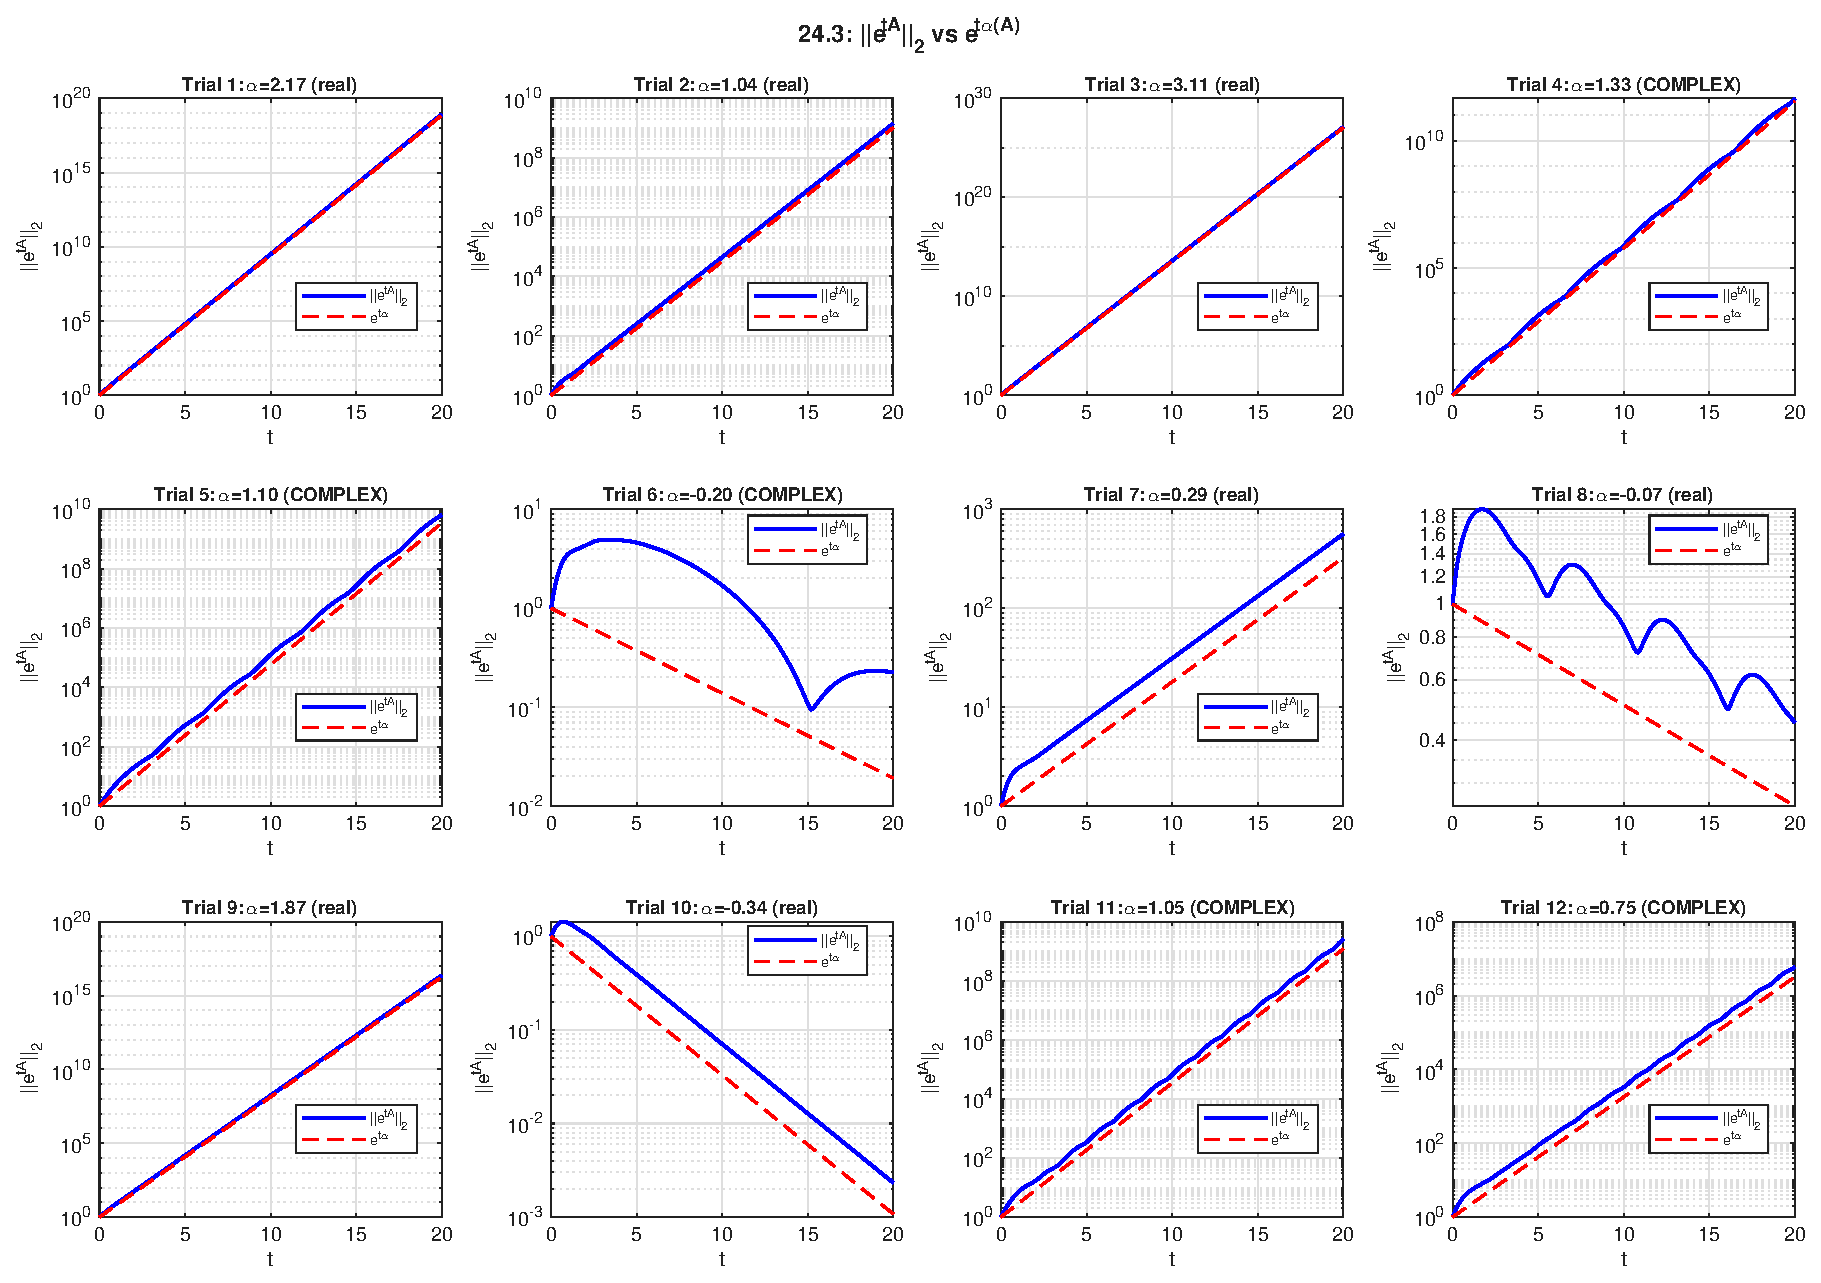
\includegraphics[width=\textwidth]{Figures/P1_main.eps}
\caption{$\|e^{tA}\|_2$ (blue) vs.\ $e^{t\alpha(A)}$ (red dashed) on a log scale for 12 trials.}
\label{fig:p1main}
\end{figure}

\begin{figure}[H]
\centering
\includegraphics[width=\textwidth]{Figures/P1_ratio.eps}
\caption{Ratio $\|e^{tA}\|_2 \,/\, e^{t\alpha(A)}$ for the same 12 trials. Titles show the dominant eigenvalue.}
\label{fig:p1ratio}
\end{figure}

\begin{itemize}
    \item In every trial, $\|e^{tA}\|_2 \geq e^{t\alpha(A)}$, so the spectral abscissa acts as a lower bound on the growth/decay rate.
    \item The ratio $\|e^{tA}\|_2 / e^{t\alpha(A)}$ settles to a finite value as $t\to\infty$, meaning $e^{t\alpha(A)}$ captures the correct asymptotic rate.
    \item Some trials show transient growth even when $\alpha(A)<0$ (e.g.\ Trials 6, 8, 10), due to the non-normality of $A$.
\end{itemize}

The curve $\|e^{tA}\|_2$ remains \emph{oscillatory} as $t\to\infty$ when the dominant eigenvalue is \textbf{complex}. In the ratio plot, trials with a complex dominant eigenvalue (e.g.\ $1.33+0.95i$, $1.10+1.10i$, $1.05+1.97i$, $0.75+2.20i$) oscillate persistently, while those with a real dominant eigenvalue flatten out. This happens because $e^{t\lambda} = e^{t\operatorname{Re}(\lambda)} \cdot e^{it\operatorname{Im}(\lambda)}$: the first factor controls growth/decay, while the second oscillates with period $2\pi/|\operatorname{Im}(\lambda)|$.

%% ============================================================
\newpage
\section{Implement-and-Test -- Householder Reduction to Hessenberg Form.}
%% ============================================================

\subsection{Problem}
Submit: Code + Validation, show working $5\times5$ and $7\times7$ examples.
Compare with a library call (e.g. \verb|hess|) --- for validation use a $9\times9$ example. Comment on similarities and differences.

\subsection{Solution}

The implementation follows Algorithm 26.1 (Trefethen \& Bau). At each step $k$, a Householder reflector $Q_k$ is chosen to leave the first $k$ rows unchanged, introducing zeros below the subdiagonal in column $k$. The right-multiplication by $Q_k$ only mixes columns $k{+}1,\ldots,m$, preserving the zeros already introduced. The result is a similarity transformation $H = Q^TAQ$ in upper Hessenberg form.

\textbf{$5\times5$ matrix:}
$$H = \begin{bmatrix}
 0.1609 & -1.3903 &  0.9019 & -0.8620 &  0.6595 \\
 1.2752 & -1.4534 & -1.5474 &  0.5078 &  1.6177 \\
 0      & -1.0510 &  0.8818 & -1.3579 & -1.3146 \\
 0      &  0      &  2.0099 & -0.5017 &  2.2336 \\
 0      &  0      &  0      & -0.2236 & -0.0437
\end{bmatrix}$$
$\|QHQ^T - A\| = 5.18\times10^{-15}$, \quad $\|Q^TQ - I\| = 1.55\times10^{-15}$.

\textbf{$7\times7$ matrix:}
$$H = \begin{bmatrix}
 1.3685 & -1.2520 &  0.6385 &  0.0816 &  0.6459 & -1.9721 &  0.2283 \\
 2.2339 & -0.1934 &  0.3656 & -0.1672 & -0.9138 & -0.1742 & -0.1961 \\
 0      &  2.6565 &  2.5680 & -0.7610 & -1.2410 & -0.0366 & -1.5187 \\
 0      &  0      & -1.5629 &  1.3058 &  1.4355 & -1.3195 &  0.6787 \\
 0      &  0      &  0      &  1.8152 &  0.7519 & -1.0083 & -0.6156 \\
 0      &  0      &  0      &  0      & -0.9047 &  0.1798 & -1.8903 \\
 0      &  0      &  0      &  0      &  0      & -1.4207 & -1.3685
\end{bmatrix}$$
$\|QHQ^T - A\| = 2.99\times10^{-15}$, \quad $\|Q^TQ - I\| = 9.45\times10^{-16}$.

\textbf{$9\times9$ validation vs.\ \texttt{hess()}:}

\begin{center}
\begin{tabular}{lcc}
\hline
 & my code & \verb|hess()| \\
\hline
$\|QHQ^T - A\|$ & $5.61\times10^{-15}$ & $2.50\times10^{-15}$ \\
$\|Q^TQ - I\|$  & $1.47\times10^{-15}$ & $7.59\times10^{-16}$ \\
max $|H_{ij}|$ below subdiag & $0$ & $0$ \\
\hline
\end{tabular}
\end{center}

The eigenvalues of $A$ and $H$ match to all displayed digits, confirming that the similarity transformation preserves the spectrum.

\textbf{Similarities:} Both produce valid upper Hessenberg matrices with $\|QHQ^T-A\| = \mathcal{O}(\varepsilon_{\mathrm{mach}})$, orthogonal $Q$, and identical eigenvalues.

\textbf{Differences:} The matrices $H$ and $Q$ are not identical between the two implementations.



%% ============================================================
\newpage
\section{Implement-and-Test -- Rayleigh Quotient Iteration.}
%% ============================================================

\subsection{Problem}
Submit: Code + Validation
Minimum Validation: $11\times11$ matrix; (explicitly) show that at least one eigenvalue-eigenvector pair matches library call in MATLAB.

\subsection{Solution}

The implementation follows Algorithm 27.3 (Trefethen \& Bau). The Rayleigh quotient $\lambda^{(k)} = v^{(k)T}\!Av^{(k)}$ gives a quadratically accurate eigenvalue estimate, and inverse iteration refines the eigenvector at each step. For real symmetric matrices, this yields cubic convergence (Theorem 27.3).

The algorithm was applied to a random $11\times11$ symmetric matrix from five starting vectors. In every case, RQI converged to an eigenvalue--eigenvector pair matching \verb|eig()| to machine precision:

\begin{center}
\begin{tabular}{cccc}
\hline
Start & Converged $\lambda$ & Lib match \# & $|\lambda_{\mathrm{RQI}} - \lambda_{\mathrm{lib}}|$ \\
\hline
1 & $-1.244051896238503$ & 5 & $1.78\times10^{-15}$ \\
2 & $\phantom{-}0.156283081516918$ & 6 & $0$ \\
3 & $-1.244051896238503$ & 5 & $1.11\times10^{-15}$ \\
4 & $\phantom{-}0.900730478209063$ & 7 & $2.22\times10^{-16}$ \\
5 & $\phantom{-}0.156283081516918$ & 6 & $1.11\times10^{-16}$ \\
\hline
\end{tabular}
\end{center}

\textbf{Eigenpair verification:}
\begin{align*}
\lambda_{\mathrm{RQI}} &= 2.828348903885657 \\
\lambda_{\mathrm{lib}} &= 2.828348903885659 \\
|\lambda_{\mathrm{RQI}} - \lambda_{\mathrm{lib}}| &= 2.22\times10^{-15} \\
\|v_{\mathrm{RQI}} - v_{\mathrm{lib}}\|_2 &= 1.64\times10^{-15} \\
\|Av - \lambda v\|_2 &= 9.50\times10^{-16}
\end{align*}

\textbf{Cubic convergence:} The table below shows $|e_k| = |\lambda^{(k)} - \lambda_{\mathrm{true}}|$ and the ratio $\log_{10}|e_k|/\log_{10}|e_{k-1}|$, which approaches 3 as predicted by Theorem 27.3:

\begin{center}
\begin{tabular}{ccc}
\hline
$k$ & $|e_k|$ & $\log|e_k|/\log|e_{k-1}|$ \\
\hline
1 & $1.5621\times10^{-1}$ & 3.09 \\
2 & $3.2118\times10^{-3}$ & 3.09 \\
3 & $2.0848\times10^{-8}$ & 3.08 \\
4 & $1.3323\times10^{-15}$ & 1.94 \\
5 & $2.2204\times10^{-15}$ & 0.99 \\
\hline
\end{tabular}
\end{center}

The ratio is approximately 3 for iterations 1--3, confirming cubic convergence. At iteration~4 the error hits machine epsilon and the ratio breaks down, which is expected. Note that the near-singular warnings from MATLAB (suppressed in code) are expected and harmless: as $\lambda^{(k)}\to\lambda_J$, the matrix $(A-\lambda^{(k)}I)$ becomes singular by definition, but this does not affect the accuracy of inverse iteration (cf.\ Exercise~27.5).

%% ============================================================
\newpage
\section*{Appendix: MATLAB Code}
%% ============================================================

\lstinputlisting{HW8.m}

%% ============================================================
\newpage
\section*{Appendix: MATLAB Output}
%% ============================================================

\begin{verbatim}
=== Problem 2: Householder Hessenberg ===

--- 5x5 ---
H =
    0.1609   -1.3903    0.9019   -0.8620    0.6595
    1.2752   -1.4534   -1.5474    0.5078    1.6177
         0   -1.0510    0.8818   -1.3579   -1.3146
         0         0    2.0099   -0.5017    2.2336
         0         0         0   -0.2236   -0.0437

||Q*H*Q'-A|| = 5.18e-15,  ||Q'Q-I|| = 1.55e-15

--- 7x7 ---
H =
    1.3685   -1.2520    0.6385    0.0816    0.6459   -1.9721    0.2283
    2.2339   -0.1934    0.3656   -0.1672   -0.9138   -0.1742   -0.1961
         0    2.6565    2.5680   -0.7610   -1.2410   -0.0366   -1.5187
         0         0   -1.5629    1.3058    1.4355   -1.3195    0.6787
         0         0         0    1.8152    0.7519   -1.0083   -0.6156
         0         0         0         0   -0.9047    0.1798   -1.8903
         0         0         0         0         0   -1.4207   -1.3685

||Q*H*Q'-A|| = 2.99e-15,  ||Q'Q-I|| = 9.45e-16

--- 9x9 Validation vs hess() ---
              Ours          hess()
||QHQ'-A||   5.61e-15    2.50e-15
||Q'Q-I||    1.47e-15    7.59e-16
max below    0.00e+00    0.00e+00

eig(A): -1.930148 -1.930148 -0.942473 -0.066067 -0.066067 1.294533 1.294533 1.446307 2.698050 
eig(H): -1.930148 -1.930148 -0.942473 -0.066067 -0.066067 1.294533 1.294533 1.446307 2.698050 

=== Problem 3: Rayleigh Quotient Iteration (11x11) ===

Library eigenvalues:
  lambda_ 1 =  -8.07026331030929
  lambda_ 2 =  -6.35514062816386
  lambda_ 3 =  -4.24037246642239
  lambda_ 4 =  -3.73156424651871
  lambda_ 5 =  -1.24405189623850
  lambda_ 6 =   0.15628308151692
  lambda_ 7 =   0.90073047820906
  lambda_ 8 =   1.60010137723812
  lambda_ 9 =   2.82834890388566
  lambda_10 =   4.94499401678928
  lambda_11 =   6.00937039025832

--- RQI runs ---
Warning: Matrix is close to singular or badly scaled. Results may be inaccurate. RCOND =  1.021050e-17. 
> In HW8>rayleigh_quotient_iteration (line 168)
In HW8 (line 112)
 
Start 1: lambda=-1.244051896238503  matches #5  |err|=1.78e-15  res=8.03e-16
Warning: Matrix is close to singular or badly scaled. Results may be inaccurate. RCOND =  1.254987e-17. 
> In HW8>rayleigh_quotient_iteration (line 168)
In HW8 (line 112)
 
Start 2: lambda=0.156283081516918  matches #6  |err|=0.00e+00  res=7.31e-16
Warning: Matrix is close to singular or badly scaled. Results may be inaccurate. RCOND =  1.021050e-17. 
> In HW8>rayleigh_quotient_iteration (line 168)
In HW8 (line 112)
 
Start 3: lambda=-1.244051896238503  matches #5  |err|=1.11e-15  res=9.13e-16
Warning: Matrix is close to singular or badly scaled. Results may be inaccurate. RCOND =  4.215812e-19. 
> In HW8>rayleigh_quotient_iteration (line 168)
In HW8 (line 112)
 
Start 4: lambda=0.900730478209063  matches #7  |err|=2.22e-16  res=6.56e-16
Warning: Matrix is close to singular or badly scaled. Results may be inaccurate. RCOND =  3.137468e-17. 
> In HW8>rayleigh_quotient_iteration (line 168)
In HW8 (line 112)
 
Start 5: lambda=0.156283081516918  matches #6  |err|=1.11e-16  res=8.15e-16

--- Detailed eigenpair verification ---
Warning: Matrix is close to singular or badly scaled. Results may be inaccurate. RCOND =  1.802876e-17. 
> In HW8>rayleigh_quotient_iteration (line 168)
In HW8 (line 122)
 
  RQI lambda  =    2.828348903885657
  Lib lambda  =    2.828348903885659
  |difference|= 2.22e-15
  ||v_rqi - v_lib|| = 1.64e-15
  ||Av - lam*v||    = 9.50e-16

  Cubic convergence:
    k=1: err=1.5621e-01  ratio=3.09
    k=2: err=3.2118e-03  ratio=3.09
    k=3: err=2.0848e-08  ratio=3.08
    k=4: err=1.3323e-15  ratio=1.94
    k=5: err=2.2204e-15  ratio=0.99
\end{verbatim}

\end{document}